The following chapter describes our understanding of Valcon as a company. This includes the environment in which they operate, an analysis of their business model, their business and IT strategies, and an identification of which work domains that affect the problem.

We conducted the analysis before realising that OMT was a big part of the problem, and therefore the analysis in regards to OMT is very limited.

\section{Business environment}
As we are working with internal support functions, we provide only summaries of our environment analyses here.
\subsection{Valcon's environment}
Valcon operates within an competitive environment where image is key. 
There's a major need for experienced and knowledgeable consultants but there's also a lot of competition in the field.
Due to this, Valcon's business strategy has been to hire the best and brightest employees and accept the fact that they're unable to be the cheapest organisation to hire,
but they pride themselves with being a company who follows their customers all the way to the finish line with the projects that they've been hired to do. 
They work hard trying to hire consultants within a wide range of fields, meaning there's a high chance that they have just the consultant a new project needs, no matter what field the project operates within. 
This means that Valcon is a company competing on quality and knowledge rather than on the price, meaning that Valcon is able to compete with other companies that might be fighting each other on the price.
\subsection{OMT's environment}
OMT operates within an environment where they aren't facing a lot of competition. 
There aren't many ship designers building war ships and this places OMT in a position where they need employees with that specific experience and there aren't many candidates, as most of these employees are most likely already employed somewhere else.
Because of this, OMT finds a lot of their workforce within other ship design companies. 
Since these other companies work in other fields where OMT doesn't, they don't mind subcontracting the employees that OMT wants, as this just gives them more work. 
\section{Valcon's business model}
The business canvas gives an overview of Valcon's business.
Based on our analysis we have the following understanding of Valcon's canvas.
\begin{figure}[!htp]
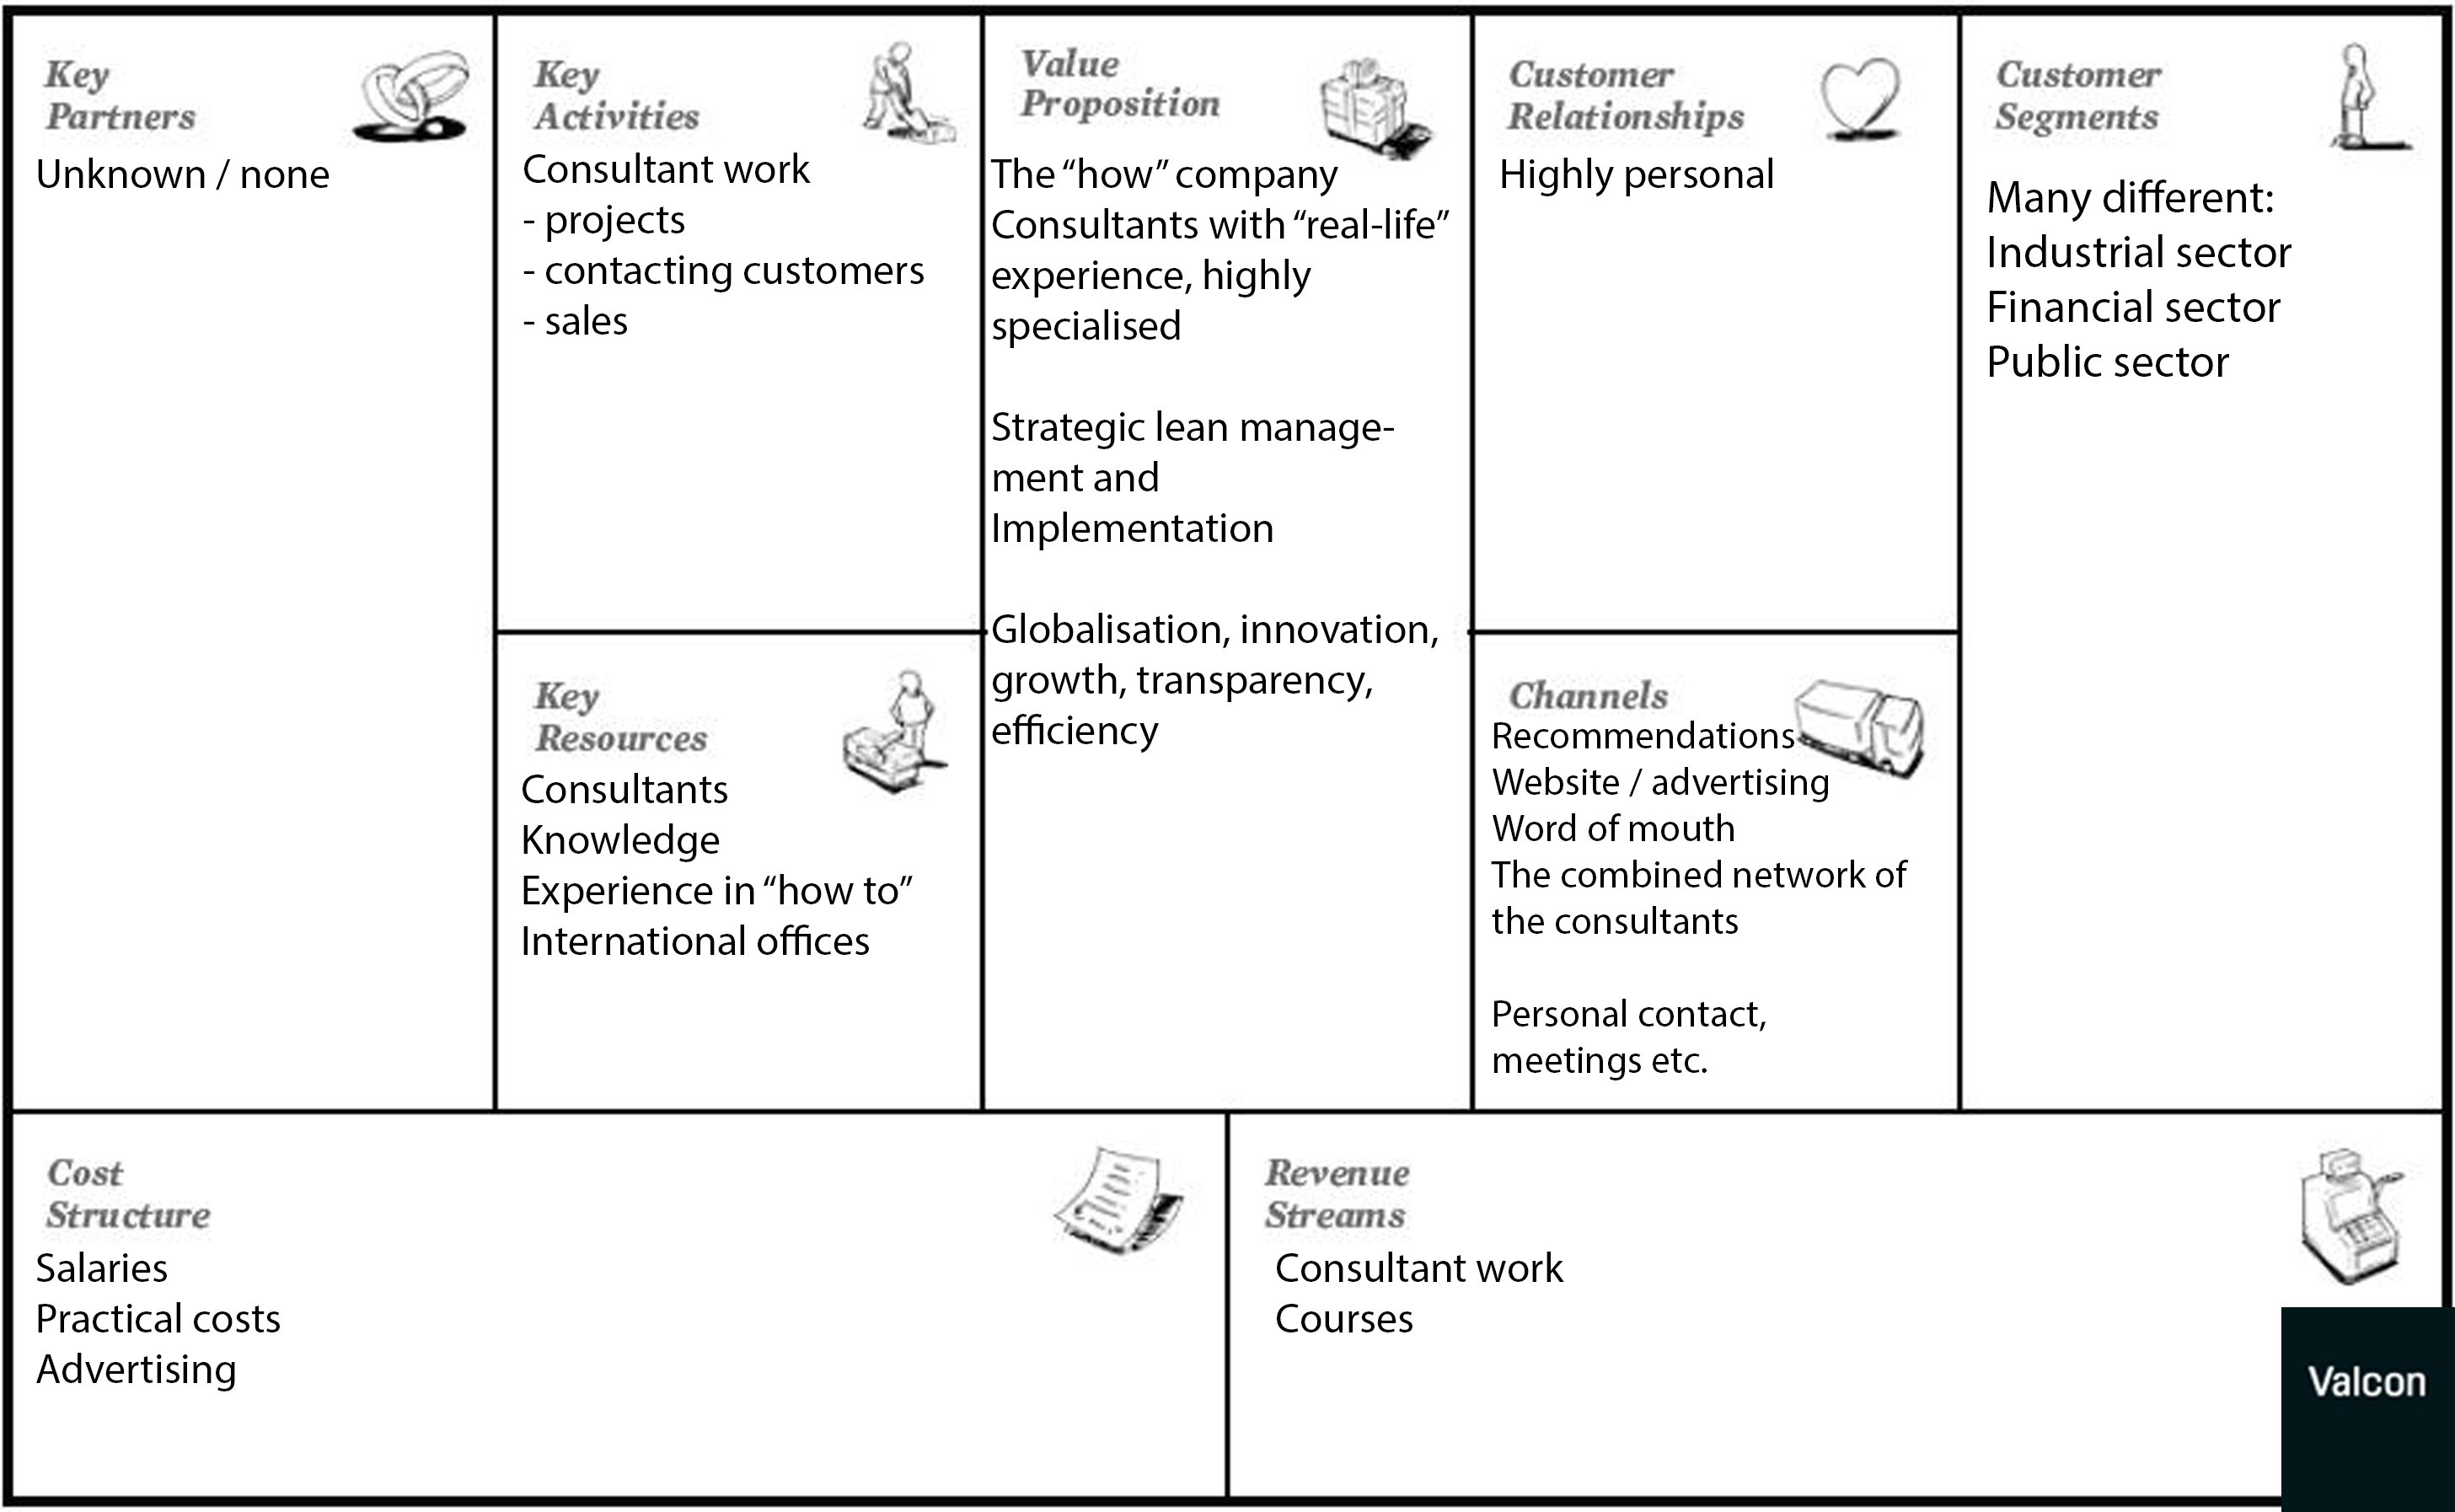
\includegraphics[width=\textwidth]{inline/business-model-canvas.png}
\caption{Valcon's business canvas.}
\label{fig:canvas}
\end{figure}

The Business Canvas gives an overview of Valcon as a whole. In relation to the problem it is important to note that the consultants are key resources for Valcon's business, as they are the ones who generate revenue.
As such it is important that they are able to perform their work effectively as soon as they start working at Valcon. It gives us a good understanding of why the company might value the consultants' time highly. (Sources: Initial meeting with Danni (appendix \ref{app:danni_initiation}), Valcon's homepage. Approved by Danni during inline conclusion meeting (appendix \ref{app:danni_inline}).) (See appendix \ref{app:canvas}.)

We have chosen not to do a canvas for OMT because \todo{Why no OMT canvas?}
\section{Business strategy, IT strategy and company values}
\subsubsection{Business strategy}
We were not able to acquire Valcon's business strategy, as it is not public and Valcon were not interested in sharing it. (Source: appendix \ref{app:business_strategy_refusal}). 
However, we were able to glean some of it through the interviews and meetings:

Valcon is in rapid growth and have a continued focus on keeping this growth as high as possible. 

(Sources: appendix \quoteref{app:danni_initiation}{danni_init_eksplosiv_vekst} and appendix \quoteref{app:danni_initiation}{danni_init_business_strategy_vekst}).

\subsubsection{IT strategy}
Valcon's IT strategy focuses on streamlining IT activities, being cost efficient, outsourcing labor intensive tasks, making work easier for the consultants, few but strong partnerships and choosing off-the-shelf systems instead of customized systems.

See appendix \ref{app:it_strategy} for the original document.

\subsubsection{Company values}
Valcon is guided by four values internally: Integrity, joy, performance, and competence.
Furthermore they value a flat hierarchy.
(Source: appendix \quoteref{app:danni_initiation}{danni_init_firmastruktur}).
\section{Work domains}
The problem involves the following work domains:

\begin{itemize}
\item \emph{OMT and Valcon recruiters} contact and acquire particulars of the new employee. They send this to accounting. \\
(Source: appendix \quoteref{app:danni_initiation}{danni_init_recruiter}).

\item \emph{Accounting} sets the employee up in the economical systems and handles the contract. \\
(Source: appendix \quoteref{app:danni_initiation}{danni_init_accounting}).

\item \emph{IT} sets the employee up in the internal systems, sets up a computer and sends it to him/her, and sometimes sets up a phone and internet connection as well. \\
(Source: appendix \quoteref{app:danni_initiation}{danni_init_IT}).

\item \emph{New employees} are contacted about contract, computer, phone, and internet information. \\
(Sources: appendix \quoteref{app:peter}{peter_stamdata} and \quoteref{app:lisbeth}{lisbeth_kontrakt}).
\end{itemize}

A visual representation of the organization as well as the work domains to investigate can be seen in appendix \ref{app:OrganizationalChart}.
\section{Conclusion}
Part of Valcon's business strategy is to maintain a high growth rate for the company.
A high growth rate means many new employees.
All employments go through Group Support Functions (IT and Accounting).

Since Valcon intends to keep growing, it is relevant to investigate whether the process needs to be optimized or not.